\documentclass{standalone}
\usepackage{tikz}
\usetikzlibrary{patterns, positioning}

\begin{document}
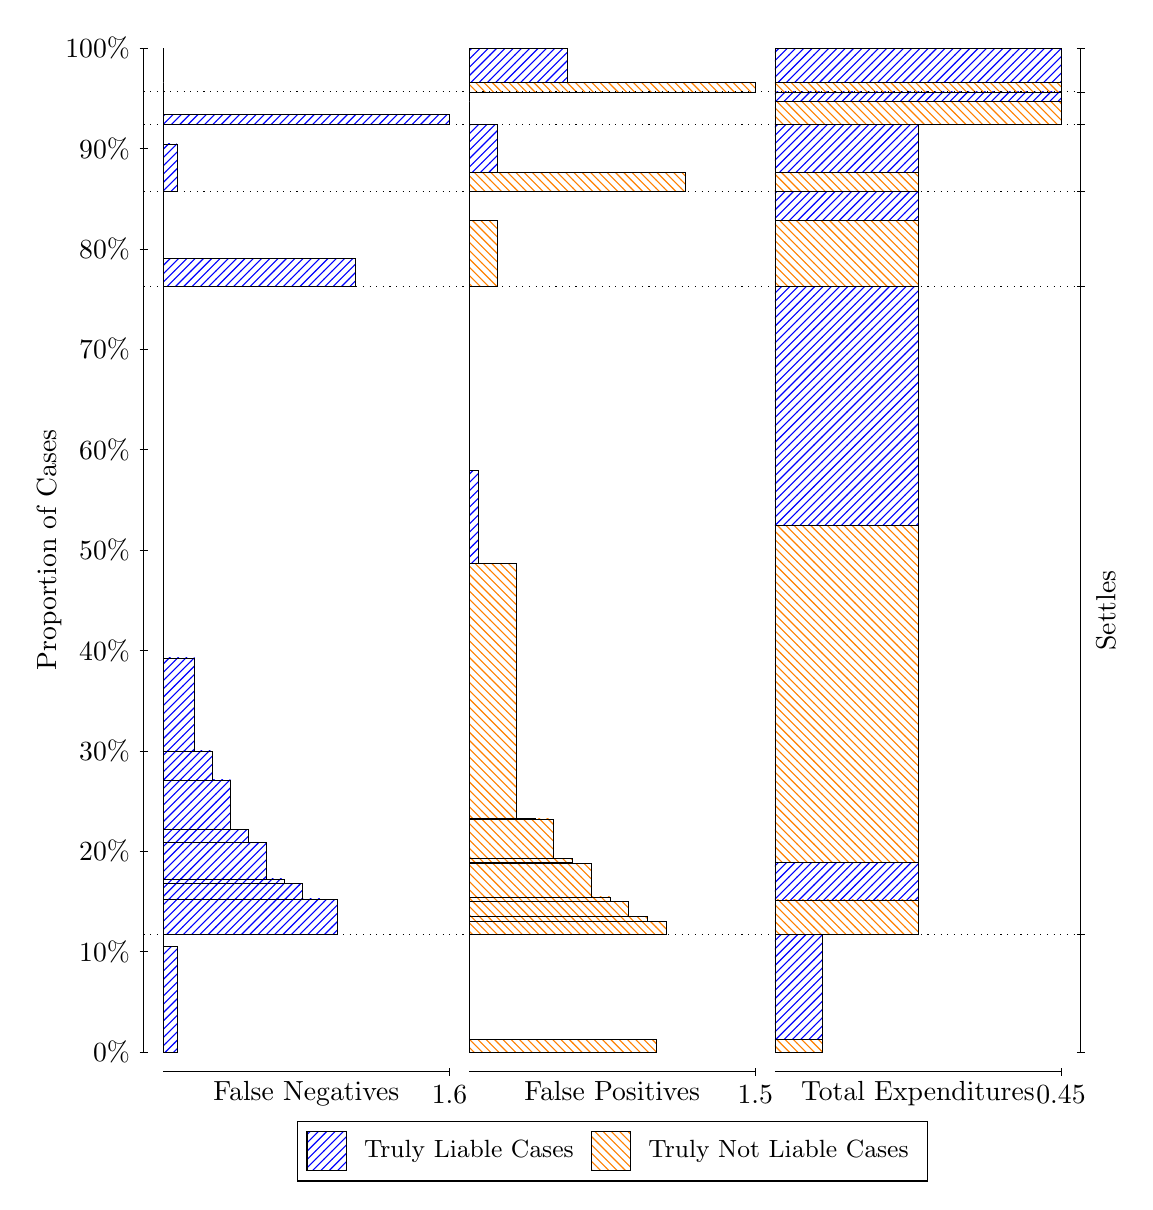
\begin{tikzpicture}
\draw[black, very thin] (1.5,1.75) -- (1.5,14.5);
\node[rotate=90, anchor=center] at (0.3, 8.125) {Proportion of Cases};
\draw[black, very thin] (1.45,1.75) -- (1.55,1.75);
\node[anchor=east] at (1.45, 1.75) {0\%};
\draw[black, very thin] (1.45,3.025) -- (1.55,3.025);
\node[anchor=east] at (1.45, 3.025) {10\%};
\draw[black, very thin] (1.45,4.3) -- (1.55,4.3);
\node[anchor=east] at (1.45, 4.3) {20\%};
\draw[black, very thin] (1.45,5.575) -- (1.55,5.575);
\node[anchor=east] at (1.45, 5.575) {30\%};
\draw[black, very thin] (1.45,6.85) -- (1.55,6.85);
\node[anchor=east] at (1.45, 6.85) {40\%};
\draw[black, very thin] (1.45,8.125) -- (1.55,8.125);
\node[anchor=east] at (1.45, 8.125) {50\%};
\draw[black, very thin] (1.45,9.4) -- (1.55,9.4);
\node[anchor=east] at (1.45, 9.4) {60\%};
\draw[black, very thin] (1.45,10.675) -- (1.55,10.675);
\node[anchor=east] at (1.45, 10.675) {70\%};
\draw[black, very thin] (1.45,11.95) -- (1.55,11.95);
\node[anchor=east] at (1.45, 11.95) {80\%};
\draw[black, very thin] (1.45,13.225) -- (1.55,13.225);
\node[anchor=east] at (1.45, 13.225) {90\%};
\draw[black, very thin] (1.45,14.5) -- (1.55,14.5);
\node[anchor=east] at (1.45, 14.5) {100\%};

\draw[black, very thin] (13.4,1.75) -- (13.4,14.5);
\draw[black, very thin] (13.35,1.75) -- (13.45,1.75);
\node[anchor=west] at (13.35, 1.75) {};
\draw[black, very thin] (13.35,3.2449) -- (13.45,3.2449);
\node[anchor=west] at (13.35, 3.2449) {};
\draw[black, very thin] (13.35,11.469) -- (13.45,11.469);
\node[anchor=west] at (13.35, 11.469) {};
\draw[black, very thin] (13.35,12.676) -- (13.45,12.676);
\node[anchor=west] at (13.35, 12.676) {};
\draw[black, very thin] (13.35,13.533) -- (13.45,13.533);
\node[anchor=west] at (13.35, 13.533) {};
\draw[black, very thin] (13.35,13.944) -- (13.45,13.944);
\node[anchor=west] at (13.35, 13.944) {};
\draw[black, very thin] (13.35,14.5) -- (13.45,14.5);
\node[anchor=west] at (13.35, 14.5) {};

\draw[black, very thin, pattern color=blue, pattern=north east lines] (1.75,1.75) rectangle (1.9203,3.0876);
\draw[black, very thin, pattern color=orange, pattern=north west lines] (1.75,3.0876) rectangle (1.75,3.2449);
\draw[black, very thin, pattern color=blue, pattern=north east lines] (1.75,3.2449) rectangle (3.9641,3.6896);
\draw[black, very thin, pattern color=blue, pattern=north east lines] (1.75,3.6896) rectangle (3.737,3.6944);
\draw[black, very thin, pattern color=blue, pattern=north east lines] (1.75,3.6944) rectangle (3.5099,3.8863);
\draw[black, very thin, pattern color=blue, pattern=north east lines] (1.75,3.8863) rectangle (3.2828,3.9493);
\draw[black, very thin, pattern color=blue, pattern=north east lines] (1.75,3.9493) rectangle (3.0557,4.4134);
\draw[black, very thin, pattern color=blue, pattern=north east lines] (1.75,4.4134) rectangle (2.8286,4.5748);
\draw[black, very thin, pattern color=blue, pattern=north east lines] (1.75,4.5748) rectangle (2.6016,5.2063);
\draw[black, very thin, pattern color=blue, pattern=north east lines] (1.75,5.2063) rectangle (2.3745,5.5752);
\draw[black, very thin, pattern color=blue, pattern=north east lines] (1.75,5.5752) rectangle (2.1474,6.754);
\draw[black, very thin, pattern color=orange, pattern=north west lines] (1.75,6.754) rectangle (1.75,11.469);
\draw[black, very thin, pattern color=blue, pattern=north east lines] (1.75,11.469) rectangle (4.1911,11.833);
\draw[black, very thin, pattern color=orange, pattern=north west lines] (1.75,11.833) rectangle (1.75,12.676);
\draw[black, very thin, pattern color=blue, pattern=north east lines] (1.75,12.676) rectangle (1.9203,13.284);
\draw[black, very thin, pattern color=orange, pattern=north west lines] (1.75,13.284) rectangle (1.75,13.533);
\draw[black, very thin, pattern color=blue, pattern=north east lines] (1.75,13.533) rectangle (5.3833,13.653);
\draw[black, very thin, pattern color=orange, pattern=north west lines] (1.75,13.653) rectangle (1.75,13.944);
\draw[black, very thin, pattern color=orange, pattern=north west lines] (1.75,13.944) rectangle (1.75,14.065);
\draw[black, very thin, pattern color=blue, pattern=north east lines] (1.75,14.065) rectangle (1.75,14.5);
\draw[black, very thin, pattern color=orange, pattern=north west lines] (5.6333,1.75) rectangle (8.0158,1.9073);
\draw[black, very thin, pattern color=blue, pattern=north east lines] (5.6333,1.9073) rectangle (5.6333,3.2449);
\draw[black, very thin, pattern color=orange, pattern=north west lines] (5.6333,3.2449) rectangle (8.135,3.4048);
\draw[black, very thin, pattern color=orange, pattern=north west lines] (5.6333,3.4048) rectangle (7.8967,3.4762);
\draw[black, very thin, pattern color=orange, pattern=north west lines] (5.6333,3.4762) rectangle (7.6585,3.6655);
\draw[black, very thin, pattern color=orange, pattern=north west lines] (5.6333,3.6655) rectangle (7.4202,3.72);
\draw[black, very thin, pattern color=orange, pattern=north west lines] (5.6333,3.72) rectangle (7.182,4.1407);
\draw[black, very thin, pattern color=orange, pattern=north west lines] (5.6333,4.1407) rectangle (6.9437,4.1555);
\draw[black, very thin, pattern color=orange, pattern=north west lines] (5.6333,4.1555) rectangle (6.9437,4.2118);
\draw[black, very thin, pattern color=orange, pattern=north west lines] (5.6333,4.2118) rectangle (6.7055,4.7098);
\draw[black, very thin, pattern color=orange, pattern=north west lines] (5.6333,4.7098) rectangle (6.4672,4.7211);
\draw[black, very thin, pattern color=orange, pattern=north west lines] (5.6333,4.7211) rectangle (6.229,7.9596);
\draw[black, very thin, pattern color=blue, pattern=north east lines] (5.6333,7.9596) rectangle (5.7525,9.1383);
\draw[black, very thin, pattern color=blue, pattern=north east lines] (5.6333,9.1383) rectangle (5.6333,11.469);
\draw[black, very thin, pattern color=orange, pattern=north west lines] (5.6333,11.469) rectangle (5.9907,12.312);
\draw[black, very thin, pattern color=blue, pattern=north east lines] (5.6333,12.312) rectangle (5.6333,12.676);
\draw[black, very thin, pattern color=orange, pattern=north west lines] (5.6333,12.676) rectangle (8.3732,12.925);
\draw[black, very thin, pattern color=blue, pattern=north east lines] (5.6333,12.925) rectangle (5.9907,13.533);
\draw[black, very thin, pattern color=orange, pattern=north west lines] (5.6333,13.533) rectangle (5.6333,13.823);
\draw[black, very thin, pattern color=blue, pattern=north east lines] (5.6333,13.823) rectangle (5.6333,13.944);
\draw[black, very thin, pattern color=orange, pattern=north west lines] (5.6333,13.944) rectangle (9.2667,14.065);
\draw[black, very thin, pattern color=blue, pattern=north east lines] (5.6333,14.065) rectangle (6.8842,14.5);
\draw[black, very thin, pattern color=orange, pattern=north west lines] (9.5167,1.75) rectangle (10.122,1.9073);
\draw[black, very thin, pattern color=blue, pattern=north east lines] (9.5167,1.9073) rectangle (10.122,3.2449);
\draw[black, very thin, pattern color=orange, pattern=north west lines] (9.5167,3.2449) rectangle (11.333,3.6804);
\draw[black, very thin, pattern color=blue, pattern=north east lines] (9.5167,3.6804) rectangle (11.333,4.1563);
\draw[black, very thin, pattern color=orange, pattern=north west lines] (9.5167,4.1563) rectangle (11.333,8.4355);
\draw[black, very thin, pattern color=blue, pattern=north east lines] (9.5167,8.4355) rectangle (11.333,11.469);
\draw[black, very thin, pattern color=orange, pattern=north west lines] (9.5167,11.469) rectangle (11.333,12.312);
\draw[black, very thin, pattern color=blue, pattern=north east lines] (9.5167,12.312) rectangle (11.333,12.676);
\draw[black, very thin, pattern color=orange, pattern=north west lines] (9.5167,12.676) rectangle (11.333,12.925);
\draw[black, very thin, pattern color=blue, pattern=north east lines] (9.5167,12.925) rectangle (11.333,13.533);
\draw[black, very thin, pattern color=orange, pattern=north west lines] (9.5167,13.533) rectangle (13.15,13.823);
\draw[black, very thin, pattern color=blue, pattern=north east lines] (9.5167,13.823) rectangle (13.15,13.944);
\draw[black, very thin, pattern color=orange, pattern=north west lines] (9.5167,13.944) rectangle (13.15,14.065);
\draw[black, very thin, pattern color=blue, pattern=north east lines] (9.5167,14.065) rectangle (13.15,14.5);
\draw[black, dotted] (1.5,3.2449) -- (13.4,3.2449);
\draw[black, dotted] (1.5,11.469) -- (13.4,11.469);
\draw[black, dotted] (1.5,12.676) -- (13.4,12.676);
\draw[black, dotted] (1.5,13.533) -- (13.4,13.533);
\draw[black, dotted] (1.5,13.944) -- (13.4,13.944);
\draw[black, very thin] (1.75,1.5) -- (5.3833,1.5);
\node[anchor=north] at (3.5667, 1.5) {False Negatives};
\draw[black, very thin] (5.3833,1.45) -- (5.3833,1.55);
\node[anchor=north] at (5.3833, 1.45) {1.6};

\draw[black, very thin] (5.6333,1.5) -- (9.2667,1.5);
\node[anchor=north] at (7.45, 1.5) {False Positives};
\draw[black, very thin] (9.2667,1.45) -- (9.2667,1.55);
\node[anchor=north] at (9.2667, 1.45) {1.5};

\draw[black, very thin] (9.5167,1.5) -- (13.15,1.5);
\node[anchor=north] at (11.333, 1.5) {Total Expenditures};
\draw[black, very thin] (13.15,1.45) -- (13.15,1.55);
\node[anchor=north] at (13.15, 1.45) {0.45};


\node[black, centered, rotate=90] at (13.72, 7.3568) {Settles};





\draw (7.449999999999999,1.5) node[draw=none] (baseCoordinate) {};
\begin{scope}[align=center]
        \matrix[scale=0.5, draw=black, below=0.5cm of baseCoordinate, nodes={draw}, column sep=0.1cm]{
            \node[rectangle, draw, minimum width=0.5cm, minimum height=0.5cm, pattern=north east lines, pattern color=blue] {}; &
            \node[draw=none, font=\small] (B) {Truly Liable Cases}; &
            \node[rectangle, draw, minimum width=0.5cm, minimum height=0.5cm, pattern=north west lines, pattern color=orange] {}; &
            \node[draw=none, font=\small] (B) {Truly Not Liable Cases}; \\
            };
\end{scope}

\end{tikzpicture}
\end{document}